\documentclass[12pt]{article}

%-----------------------------------------------------------------------------------------------------------------------------------------
%------------------------------------------------------------Coisas essenciais------------------------------------------------------------
%-----------------------------------------------------------------------------------------------------------------------------------------

%\usepackage[utf8]{inputenc}
\usepackage{textcomp}
\usepackage[T1]{fontenc}
\usepackage[portuguese]{babel}
\usepackage[margin=1in]{geometry}
\usepackage{amsmath}
\usepackage{hyperref}
\usepackage{amssymb}
\usepackage{fancyhdr}
\usepackage{enumitem}
\usepackage{caption}
\usepackage{graphicx}
\usepackage{xcolor}
\usepackage{titlesec}
\usepackage{float}
\usepackage{fontspec}
\usepackage{tikz}
\usepackage{eso-pic}
\usepackage{background}
\usepackage{wallpaper}
\usepackage{everypage}
\usepackage{minted}
\usepackage{listings}
\usepackage{lipsum}


\lstset{
    basicstyle=\ttfamily\small,
    breaklines=true,
    frame=single
}

% Fonte
\setmainfont[BoldFont = {SourceSansPro-Bold.ttf}]{SourceSansPro-Light.ttf}

% Background das páginas
\backgroundsetup{scale=1,angle=0,opacity=1,contents={\includegraphics[width=\paperwidth,height=\paperheight]{../Imagens/FundoPagina.png}}}

% Títulos personalizados
\titleformat{\section}[block]{\Large\bfseries\color{azulgepc}}{\thesection}{1em}{}
\titleformat{\subsection}[block]{\large\bfseries\color{vermelhogepc}}{\thesubsection}{1em}{}

% Cores
\definecolor{azulgepc}{RGB}{7,36,60}
\definecolor{vermelhogepc}{RGB}{235,22,52}



\begin{document}

% Capa
\newpage
\NoBgThispage
\ThisCenterWallPaper{1}{../Imagens/CapaGEPC.png}
\thispagestyle{empty}
\pagecolor{azulgepc}
\vspace*{\fill}

{\begin{figure}[h!]
\centering
\includegraphics[width=0.3\textwidth]{../Imagens/gepc.png}
\end{figure}
\vspace{1mm}
\centering\large\textbf{\color{vermelhogepc}{Grupo de Estudos em Programação Competitiva}}\par

\centering\Huge\textbf{\color{white}{MATERIAL TEÓRICO: \\FUNDAMENTOS DA PROGRAMAÇÃO}}\par

}

\vfill
{
\centering\Large\textbf{\color{vermelhogepc}{REALIZAÇÃO:}\\
\begin{figure}[h!]
    \centering
    \begin{minipage}[t]{0.3\textwidth}
        \centering
        
\includegraphics[width=\textwidth]{../Imagens/petengcomp.png}
    \end{minipage}
    \hspace{3cm} % Adds horizontal space between minipages
    \begin{minipage}[t]{0.3\textwidth}
        \centering
        
\includegraphics[width=\textwidth]{../Imagens/petcomp.png}
    \end{minipage}
\end{figure}
}
}
\newpage


%============================================================================================================================================

% INÍCIO DO MATERIAL
\section{Introdução ao Capítulo}
Antes de mergulharmos em técnicas avançadas e problemas mais desafiadores, precisamos dominar o básico. É a partir desses fundamentos que toda a lógica de programação se constrói, independentemente da linguagem escolhida. Mesmo que pareçam simples no início, são eles que vão sustentar seu aprendizado daqui pra frente. Afinal, não existe construção sólida sem bons alicerces.

\section{Estruturas Condicionais}
Nem sempre o fluxo de instruções do nosso algoritmo serão contínuas. Às vezes, queremos que o computador realize determinada tarefa somente caso uma condição seja atendida. Por exemplo, em um sistema de banco, o usuário não pode sacar dinheiro caso sua conta não possua o valor solicitado. Para fazer esse tipo de fluxo, utilizaremos as \textbf{Estruturas Condicionais}.
\subsection{Operadores Lógicos}
Antes de explorarmos as estruturas condicionais propriamente ditas, precisamos analisar os operadores lógicos. \\
Se lembrarmos dos operadores aritméticos, como soma e multiplicação, veremos que as operações resultam em valores numéricos, do mesmo tipo que os operandos, por exemplo, em: 
\begin{lstlisting}[language=C++]
int x = 10;
int y = 20;
int res = x + y;
\end{lstlisting}
O resultado, \textit{res}, será uma variável do tipo inteiro. \\
Os operadores lógicos, por outro lado, são operadores que nos retornam valores \textit{lógicos}, ou \textit{booleanos}, como você preferir chamar. Por exemplo, o código:

\begin{lstlisting}[language=C++]
bool a = true;
bool b = false;
bool res = x && y;

\end{lstlisting}
Opera com variáveis booleanas. Vamos explorar todos os operadores:
\begin{enumerate}
    \item \textbf{AND (\&\&)}: Resulta em \textbf{true} caso ambos os valores sejam true, resulta em \textbf{false} caso contrário. e.g.:
    \begin{lstlisting}[language=C++]
        bool res;
        bool v1 = true;
        bool f1 = false;
        bool v2 = true;
        
        res = v1 && v2; // res é true
        res = v1 && f1; // res é false
    \end{lstlisting}
    \item \textbf{OR (||)}: Retorna \textbf{true} caso \textbf{pelo menos um} dos valores seja true, retorna \textbf{false} caso contrário. e.g.:
    \begin{lstlisting}[language=C++]
        bool res;
        bool v1 = true;
        bool f1 = false;
        bool v2 = true;
        bool f2 = false;
        
        res = v1 || f1; // res é true
        res = v1 || v2; // res é true
        res = f1 || f2; // res é false
    \end{lstlisting}
    \item \textbf{NOT (!)}: Opera sobre um único valor. Inverte seu valor lógico. e.g.:
    \begin{lstlisting}[language=C++]
        bool res;
        bool v1 = true;
        bool f1 = false;

        res = !v1; // res é false
        res = !f1; // res é true
    \end{lstlisting}
\end{enumerate}
Além destes, em que operamos apenas sobre valores lógicos, podemos também comparar valores numéricos, usando os operadores lógicos de comparação:
\begin{itemize}
    \item \textbf{EQUALS (==)}: Compara dois valores, caso sejam iguais, retorna \textit{true}. Caso contrário, retorna \textit{false}. e.g.:
    \begin{lstlisting}[language=C++]
        bool res;
        double valor1 = 10.3;
        double valor2 = 12.7;
        double valorIgualAo1 = 10.3;

        res = valor1 == valor2 // res é false
        res = valor1 == valorIgualAo1; // res é true
    \end{lstlisting}
    \textbf{OBS: Não confundir "=" (operador de ATRIBUIÇÃO) com "==" (operador de COMPARAÇÃO)}
    \item \textbf{GREATER THAN (>) e GREATER-EQUAL (>=)}: No caso do \textit{greater than}, resulta em \textit{true} se o primeiro valor for \textit{maior} que o segundo. Para o \textit{greater-equal}, retorna \textit{true} caso o se o primeiro valor for \textit{maior ou igual} ao segundo. e.g.:
    \begin{lstlisting}[language=C++]
        bool res;
        double valor1 = 10.3;
        double valor2 = 12.7;
        double valorIgualAo1 = 10.3;

        res = valor1 > valor2 // res é false
        res = valor2 > valor1; // res é true
        res = valor1 > valorIgualAo1; // res é false
        res = valor1 >= valorIgualAo1; // res é true
    \end{lstlisting}
    \item \textbf{LOWER THAN (<) e LOWER-EQUAL (<=)}: Operadores duais de greater-than e greater-equal. Retornam \textit{true} se o primeiro valor for menor que o segundo e menor ou igual, respectivamente. e.g.:
    \begin{lstlisting}[language=C++]
        bool res;
        double valor1 = 10.3;
        double valor2 = 12.7;
        double valorIgualAo1 = 10.3;

        res = valor1 < valor2 // res é true
        res = valor2 < valor1; // res é false
        res = valor1 < valorIgualAo1; // res é false
        res = valor1 <= valorIgualAo1; // res é true
    \end{lstlisting}
\end{itemize}

\subsection{If-else}
Com os operadores lógicos em mãos, agora podemos explorar as estruturas condicionais propriamente ditas. A estrutura \textbf{if-else} permite que o programa tome decisões: caso uma condição seja verdadeira, um bloco de código é executado; caso contrário, outro bloco pode ser executado.

A sintaxe básica em C++ é:

\begin{lstlisting}[language=C++]
if (condicao) {
    // bloco executado se condicao for true
} else {
    // bloco executado se condicao for false
}
\end{lstlisting}

O bloco \texttt{else} é opcional. Caso não haja necessidade de tratar o caso falso, podemos omiti-lo:

\begin{lstlisting}[language=C++]
int saldo = 100;
int saque = 150;

if (saldo >= saque) {
    cout << "Saque realizado com sucesso!" << endl;
}
\end{lstlisting}

Também é possível encadear múltiplas condições usando \textbf{else if}:

\begin{lstlisting}[language=C++]
double nota = 7.5;

if (nota >= 7) {
    cout << "Aprovado!" << endl;
} else if (nota >= 4 && nota < 7) {
    cout << "Avaliação Final" << endl;
} else {
    cout << "Reprovado" << endl;
}
\end{lstlisting}

Note que as condições são avaliadas de cima para baixo, e somente o primeiro bloco cuja condição seja verdadeira será executado. Portanto, a ordem das condições importa.

Também podemos combinar os operadores lógicos vistos anteriormente para criar condições mais complexas:

\begin{lstlisting}[language=C++]
int idade = 20;
bool temCarteira = true;

if (idade >= 18 && temCarteira) {
    cout << "Pode dirigir." << endl;
} else {
    cout << "Nao pode dirigir." << endl;
}
\end{lstlisting}

%============================================================================================================================================

\section{Estruturas de Repetição}
Muitas vezes, precisamos que o computador repita uma mesma tarefa várias vezes. Imagine que você queira imprimir os números de 1 a 1000: seria inviável escrever mil instruções \texttt{cout} uma a uma. Para isso, existem as \textbf{Estruturas de Repetição}, também chamadas de \textit{loops}, que nos permitem executar um bloco de código repetidamente, de forma controlada.

\subsection{For-loop}

O \textbf{for} é a estrutura de repetição mais utilizada quando sabemos, de antemão, quantas vezes o bloco deve ser executado. Sua sintaxe em C++ é:

\begin{lstlisting}[language=C++]
for (inicializacao; condicao; incremento) {
    // bloco a ser repetido
}
\end{lstlisting}

Os três componentes do \texttt{for} funcionam da seguinte maneira:
\begin{itemize}
    \item \textbf{Inicialização}: executada uma única vez, antes do loop começar. Geralmente declara e inicializa um inteiro que funcionará como contador.
    \item \textbf{Condição}: verificada antes de cada iteração. Enquanto for \textit{true}, o loop continua.
    \item \textbf{Incremento}: executado ao final de cada iteração. Geralmente atualiza o contador.
\end{itemize}

Por exemplo, para imprimir os números de 1 a 10:

\begin{lstlisting}[language=C++]
for (int i = 1; i <= 10; i++) {
    cout << i << endl;
}
\end{lstlisting}

Também podemos iterar de forma decrescente, ou com passos diferentes de 1:

\begin{lstlisting}[language=C++]
// Imprime 10, 8, 6, 4, 2
for (int i = 10; i >= 2; i -= 2) {
    cout << i << endl;
}
\end{lstlisting}

É possível ainda aninhar \texttt{for}s, criando loops dentro de loops. Isso é muito útil para percorrer matrizes, como veremos mais adiante:

\begin{lstlisting}[language=C++]
for (int i = 1; i <= 3; i++) {
    for (int j = 1; j <= 3; j++) {
        cout << i << " x " << j << " = " << i * j << endl;
    }
}
\end{lstlisting}

A análise de cada iteração, ou seja, cada vez que o bloco dentro de uma estrutura de repetição é executado, e das mudanças na variável de controle \textbf{i}, fica a cargo do leitor. Inclusive, recomendamos a prática para o aprendizado.

\subsection{While-loop}

O \textbf{while} é utilizado quando não sabemos exatamente quantas vezes o bloco deve se repetir, mas sabemos a condição que deve ser satisfeita para que o loop continue. Sua sintaxe é:

\begin{lstlisting}[language=C++]
while (condicao) {
    // bloco a ser repetido
}
\end{lstlisting}

Enquanto a condição for verdadeira, o bloco é executado. Quando se tornar falsa, o loop termina. Por exemplo, o código abaixo lê números do usuário até que ele digite zero:

\begin{lstlisting}[language=C++]
int numero;
cin >> numero;

while (numero != 0) {
    cout << "Voce digitou: " << numero << endl;
    cin >> numero;
}

cout << "Loop encerrado." << endl;
\end{lstlisting}

\textbf{Atenção}: é preciso garantir que a condição eventualmente se torne falsa, caso contrário o programa entrará em um \textbf{loop infinito} e nunca terminará.

\subsection{Do-while}

O \textbf{do-while} é semelhante ao \texttt{while}, com uma diferença fundamental: o bloco de código é executado \textbf{pelo menos uma vez}, pois a condição só é verificada ao final de cada iteração. Sua sintaxe é:

\begin{lstlisting}[language=C++]
do {
    // bloco a ser repetido
} while (condicao);
\end{lstlisting}

Isso é útil quando queremos garantir que o bloco execute ao menos uma vez independentemente da condição. Um exemplo clássico é a validação de entrada do usuário:

\begin{lstlisting}[language=C++]
int opcao;

do {
    cout << "Digite uma opcao entre 1 e 5: ";
    cin >> opcao;
} while (opcao < 1 || opcao > 5);

cout << "Opcao valida: " << opcao << endl;
\end{lstlisting}

Na figura \ref{fig:while}, há uma imagem ilustrativa para esclarecer, de forma visual, a diferença do funcionamento entre os loops \textbf{while} e \textbf{do-while}.
\begin{figure}[ht!]
    \centering
    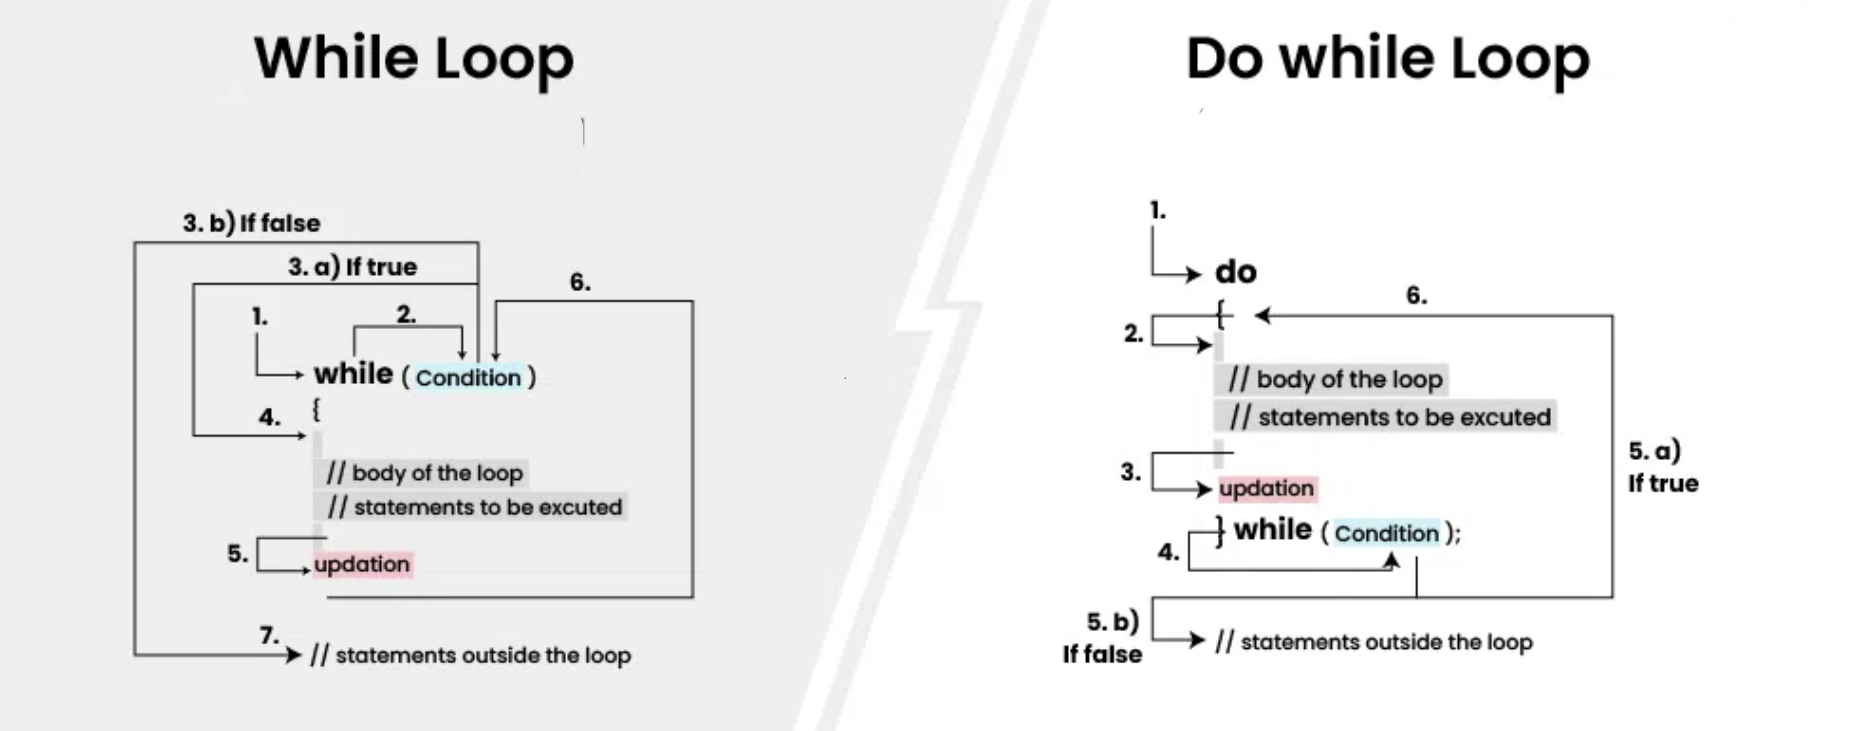
\includegraphics[width=\linewidth]{images/while.png}
    \caption{Diferença entre while-loop e do-while-loop. Fonte: GeeksforGeeks}
    \label{fig:while}
\end{figure}

%============================================================================================================================================

\section{Vetores e Matrizes}
Até agora, trabalhamos com variáveis que armazenam um único valor. Mas e quando precisamos armazenar uma coleção de valores? Imagine guardar as notas de 100 alunos: criar uma variável para cada um seria impraticável. Para isso, utilizamos \textbf{Vetores} e \textbf{Matrizes}, estruturas que nos permitem armazenar múltiplos valores em uma única variável.

\subsection{Vetores}

Um \textbf{vetor} (ou \textit{array}) é uma sequência de elementos do mesmo tipo, armazenados em posições contíguas de memória,como na figura \ref{fig:array}: 

\begin{figure}[ht!]
    \centering
    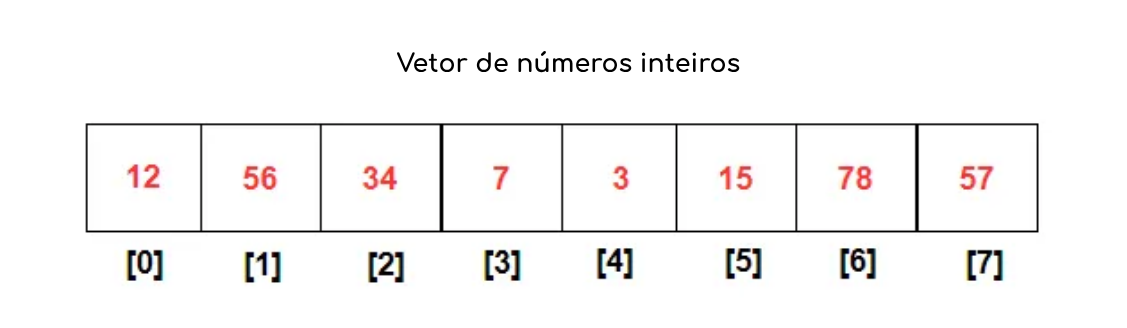
\includegraphics[width=\linewidth]{images/array.png}
    \caption{Ilustração de um vetor.}
    \label{fig:array}
\end{figure}

Para declarar um vetor em C++:

\begin{lstlisting}[language=C++]
tipo nome[tamanho];
\end{lstlisting}

Por exemplo, para declarar um vetor de 5 inteiros:

\begin{lstlisting}[language=C++]
int notas[5];
\end{lstlisting}

Podemos também inicializar o vetor na declaração:

\begin{lstlisting}[language=C++]
int notas[5] = {8, 7, 10, 6, 9};
\end{lstlisting}

O acesso aos elementos é feito por meio de um \textbf{índice}, que começa sempre em \textbf{0}:

\begin{lstlisting}[language=C++]
int notas[5] = {8, 7, 10, 6, 9};

cout << notas[0]; // imprime 8
cout << notas[2]; // imprime 10
notas[4] = 5;     // altera o ultimo elemento para 5
\end{lstlisting}

\textbf{OBS}: Acessar um índice fora dos limites do vetor (como \texttt{notas[5]} no exemplo acima) é um erro grave e pode causar comportamento inesperado no programa.

Para percorrer todos os elementos de um vetor, geralmente utilizamos um \texttt{for}:

\begin{lstlisting}[language=C++]
int notas[5] = {8, 7, 10, 6, 9};
int soma = 0;

for (int i = 0; i < 5; i++) {
    soma += notas[i];
}

cout << "Soma: " << soma << endl; // Soma: 40
\end{lstlisting}

\subsection{Strings}

Uma \textbf{string} é, essencialmente, uma sequência de caracteres. Em C++, podemos trabalhar com strings de duas formas: usando o tipo primitivo \texttt{char[]}, ou seja, um vetor de variáveis do tipo caracter, ou usando a classe \texttt{string} da biblioteca padrão, que é muito mais conveniente. Na figura \ref{fig:string}, podemos visualizar uma string no formato de vetor.

\begin{figure}[ht!]
    \centering
    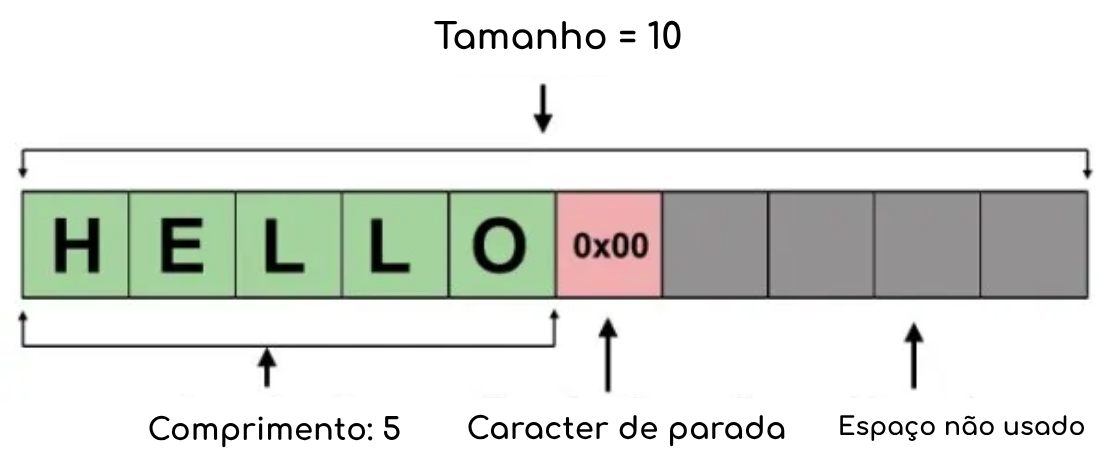
\includegraphics[width=\linewidth]{images/string.png}
    \caption{Ilustração de uma string como vetor de caracteres.}
    \label{fig:string}
\end{figure}
Vale mencionar que toda string tem um \textbf{caracter de parada} nulo após todos os caracteres significativos, ou seja, caracteres que incluímos em nossa variável. Não se preocupe com isso, uma vez que a biblioteca string fará as manipulações necessárias automaticamente.

\begin{lstlisting}[language=C++]
#include <string>

string nome = "GEPC";
cout << nome << endl;          // imprime GEPC
cout << nome.length() << endl; // imprime 4
cout << nome[0] << endl;       // imprime G
\end{lstlisting}

Assim como vetores, podemos acessar cada caractere de uma string pelo seu índice. Além disso, a classe \texttt{string} oferece diversas funções úteis:

\begin{lstlisting}[language=C++]
string s = "programacao";

cout << s.length();        // tamanho: 11
cout << s.substr(0, 7);    // subcadeia: "program"
cout << s.find("cao");     // posicao de "cao": 8

s = s + " competitiva";    // concatenacao
cout << s;                 // "programacao competitiva"
\end{lstlisting}

Para ler uma string com espaços da entrada padrão, devemos usar \texttt{getline} em vez de \texttt{cin}:

\begin{lstlisting}[language=C++]
string frase;
getline(cin, frase);
cout << frase << endl;
\end{lstlisting}

\subsection{Matrizes}

Uma \textbf{matriz} é, essencialmente, um vetor de vetores: uma estrutura bidimensional organizada em linhas e colunas. Na figura \ref{fig:matriz}, podemos visualizar uma matriz \textbf{nxn} de \textbf{n} linhas e \textbf{n} colunas. É recomendável que o leitor se habitue em entender \textbf{n} como um tamanho qualquer para um vetor ou matriz.

\begin{figure}[ht!]
    \centering
    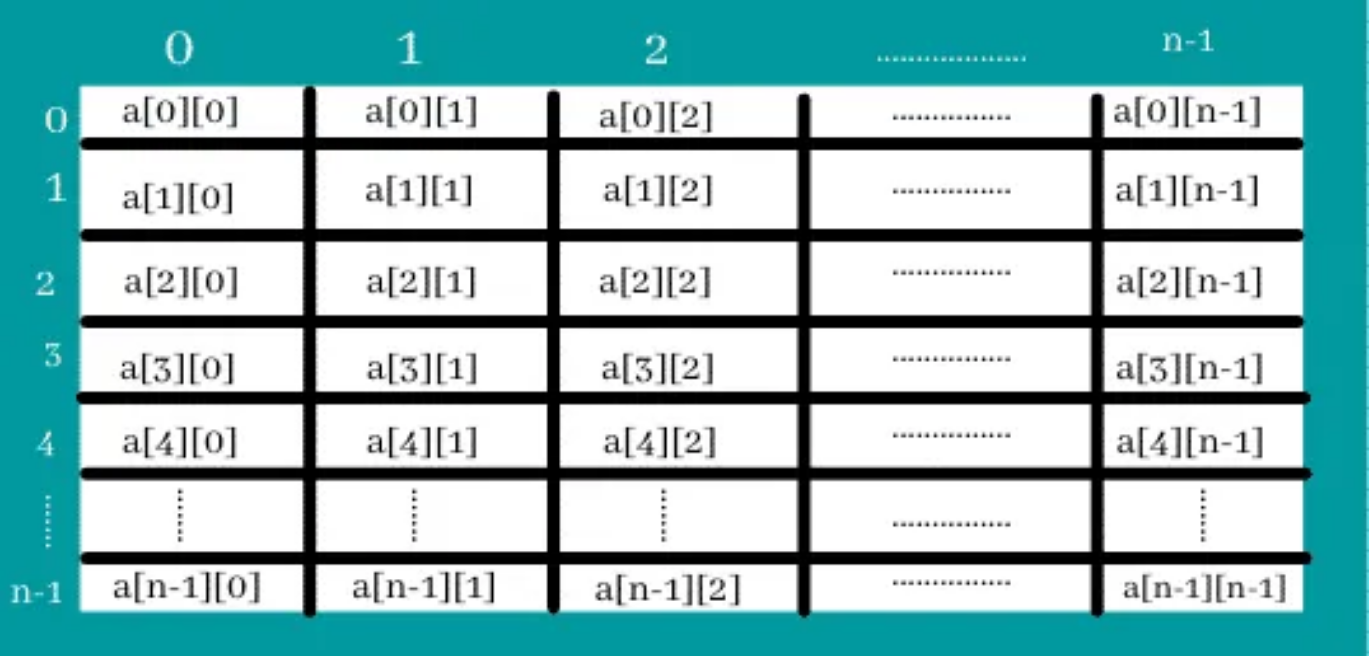
\includegraphics[width=\linewidth]{images/matriz.png}
    \caption{Ilustração de matriz nxn}
    \label{fig:matriz}
\end{figure}

 Em C++, declaramos uma matriz da seguinte forma:

\begin{lstlisting}[language=C++]
tipo nome[linhas][colunas];
\end{lstlisting}

Por exemplo, uma matriz 3x3 de inteiros:

\begin{lstlisting}[language=C++]
int mat[3][3] = {
    {1, 2, 3},
    {4, 5, 6},
    {7, 8, 9}
};
\end{lstlisting}

O acesso aos elementos é feito com dois índices: o da linha e o da coluna, ambos começando em 0:

\begin{lstlisting}[language=C++]
cout << mat[0][0]; // imprime 1 (linha 0, coluna 0)
cout << mat[1][2]; // imprime 6 (linha 1, coluna 2)
mat[2][1] = 99;    // altera o elemento da linha 2, coluna 1
\end{lstlisting}

Para percorrer todos os elementos de uma matriz, utilizamos dois \texttt{for}s aninhados:

\begin{lstlisting}[language=C++]
int mat[3][3] = {
    {1, 2, 3},
    {4, 5, 6},
    {7, 8, 9}
};

for (int i = 0; i < 3; i++) {
    for (int j = 0; j < 3; j++) {
        cout << mat[i][j] << " ";
    }
    cout << endl;
}
\end{lstlisting}

%============================================================================================================================================

\section{Funções}
À medida que nossos programas crescem, é natural que alguns trechos de código precisem ser repetidos em vários lugares. Reescrever o mesmo código diversas vezes é ineficiente e dificulta a manutenção. Para resolver isso, utilizamos \textbf{Funções}: blocos de código nomeados que realizam uma tarefa específica e podem ser chamados sempre que necessário.

\subsection{Declarando e usando funções}

A declaração de uma função em C++ segue a seguinte estrutura:

\begin{lstlisting}[language=C++]
tipo_retorno nome_funcao(tipo param1, tipo param2, ...) {
    // corpo da funcao
    return valor; // se tipo_retorno nao for void
}
\end{lstlisting}

O \textbf{tipo de retorno} indica qual tipo de valor a função devolve ao chamador. Entenda "devolver" como atribuir um valor de certo tipo, como inteiro ou booleano, e, sobre o "chamador", iremos explicar melhor sobre como chamar uma função mais adiante. Caso a função não precise retornar nenhum valor, utilizamos \texttt{void}. Os \textbf{parâmetros} são variáveis que a função recebe como entrada. Por exemplo:

\begin{lstlisting}[language=C++]
// funcao para somar dois inteiros
int soma(int a, int b) {
    return a + b;
}

// funcao para imprimir uma mensagem qualquer
void imprimirMensagem(string mensagem) {
    cout << mensagem << endl;
}
\end{lstlisting}

Para usar (chamar) uma função, basta escrever seu nome seguido dos argumentos:

\begin{lstlisting}[language=C++]
int resultado = soma(3, 7);
cout << resultado << endl; // imprime 10

imprimirMensagem("Ola, GEPC!"); // imprime Ola, GEPC!
\end{lstlisting}

Em C++, uma função precisa ser declarada \textbf{antes} de ser chamada. Caso queira definir a função depois do \texttt{main}, é necessário escrever seu \textbf{protótipo} antes:

\begin{lstlisting}[language=C++]
int soma(int a, int b); // prototipo

int main() {
    cout << soma(4, 6) << endl;
    return 0;
}

int soma(int a, int b) { // definicao
    return a + b;
}
\end{lstlisting}

\subsection{Recursividade}

Uma função é dita \textbf{recursiva} quando ela chama a si mesma dentro do próprio corpo. Essa técnica é muito poderosa e nos permite resolver problemas que possuem uma estrutura naturalmente repetitiva ou que podem ser divididos em subproblemas menores do mesmo tipo.

Toda função recursiva precisa de dois elementos fundamentais:
\begin{itemize}
    \item \textbf{Caso base}: a condição de parada, que define quando a função deve parar de chamar a si mesma.
    \item \textbf{Caso recursivo}: a chamada da função a si mesma, reduzindo o problema a cada passo.
\end{itemize}

O exemplo clássico de recursividade é o cálculo do \textbf{fatorial}. Sabemos que $n! = n \times (n-1)!$, com $0! = 1$:

\begin{lstlisting}[language=C++]
int fatorial(int n) {
    if (n == 0) return 1;       // caso base
    return n * fatorial(n - 1); // caso recursivo
}

int main() {
    cout << fatorial(5) << endl; // imprime 120
    return 0;
}
\end{lstlisting}

Outro exemplo clássico é o cálculo do \textbf{$n$-ésimo termo da sequência de Fibonacci}, definida por $F(0) = 0$, $F(1) = 1$ e $F(n) = F(n-1) + F(n-2)$:

\begin{lstlisting}[language=C++]
int fibonacci(int n) {
    if (n == 0) return 0;                        // caso base
    if (n == 1) return 1;                        // caso base
    return fibonacci(n - 1) + fibonacci(n - 2); // caso recursivo
}
\end{lstlisting}

\textbf{Atenção}: toda função recursiva deve garantir que o caso base seja atingido em algum momento. Caso contrário, a função chamará a si mesma indefinidamente, causando um \textit{stack overflow} e travando o programa.\\

\vspace{5mm}

Em exemplos como o da sequência de fibonacci, a sintaxe do método recursivo é bem mais intuitiva e legível do que utilizando loops. Fica como exercício para o leitor resolver alguma questão sobre loops utilizando uma função recursiva.

\end{document}
